\hypertarget{group__BEEPER}{\section{Beeper}
\label{group__BEEPER}\index{Beeper@{Beeper}}
}


Beeper is used for auditory indication of various states and events.  


Collaboration diagram for Beeper\+:\nopagebreak
\begin{figure}[H]
\begin{center}
\leavevmode
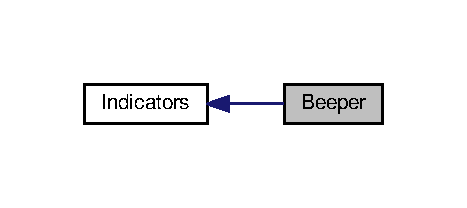
\includegraphics[width=224pt]{group__BEEPER}
\end{center}
\end{figure}
Beeper is used for auditory indication of various states and events. 

The role of the beeper module is to provide a more advanced interface to the system beeper function (which can only turn the beeper on or off). This module provides several standard beep sequences that can be started by user code and run asynchronously by periodically calling the update function. 